\documentclass{article}
\usepackage{yfonts, xcolor}
\usepackage[object=vectorian]{pgfornament}
\usepackage{eso-pic}
\usepackage{geometry}
\geometry{
 a4paper,
 total={170mm,257mm},
 left=25mm,
 right=25mm,
 top=25mm,
}
% Page background taken from here: https://latex.org/forum/viewtopic.php?f=5&t=25013

\usetikzlibrary{calc}
\renewcommand{\labelitemi}{\labelitemfont\textbf{\textdagger}}
\renewcommand{\labelitemii}{\labelitemfont\textbf{\textendash}}
\pagenumbering{gobble}

\graphicspath{ {./Images/} }

\begin{document}
\AddToShipoutPicture{\put(0,0){\includegraphics[width=\paperwidth, height=\paperheight]{odd_page.jpg}}}
\centering
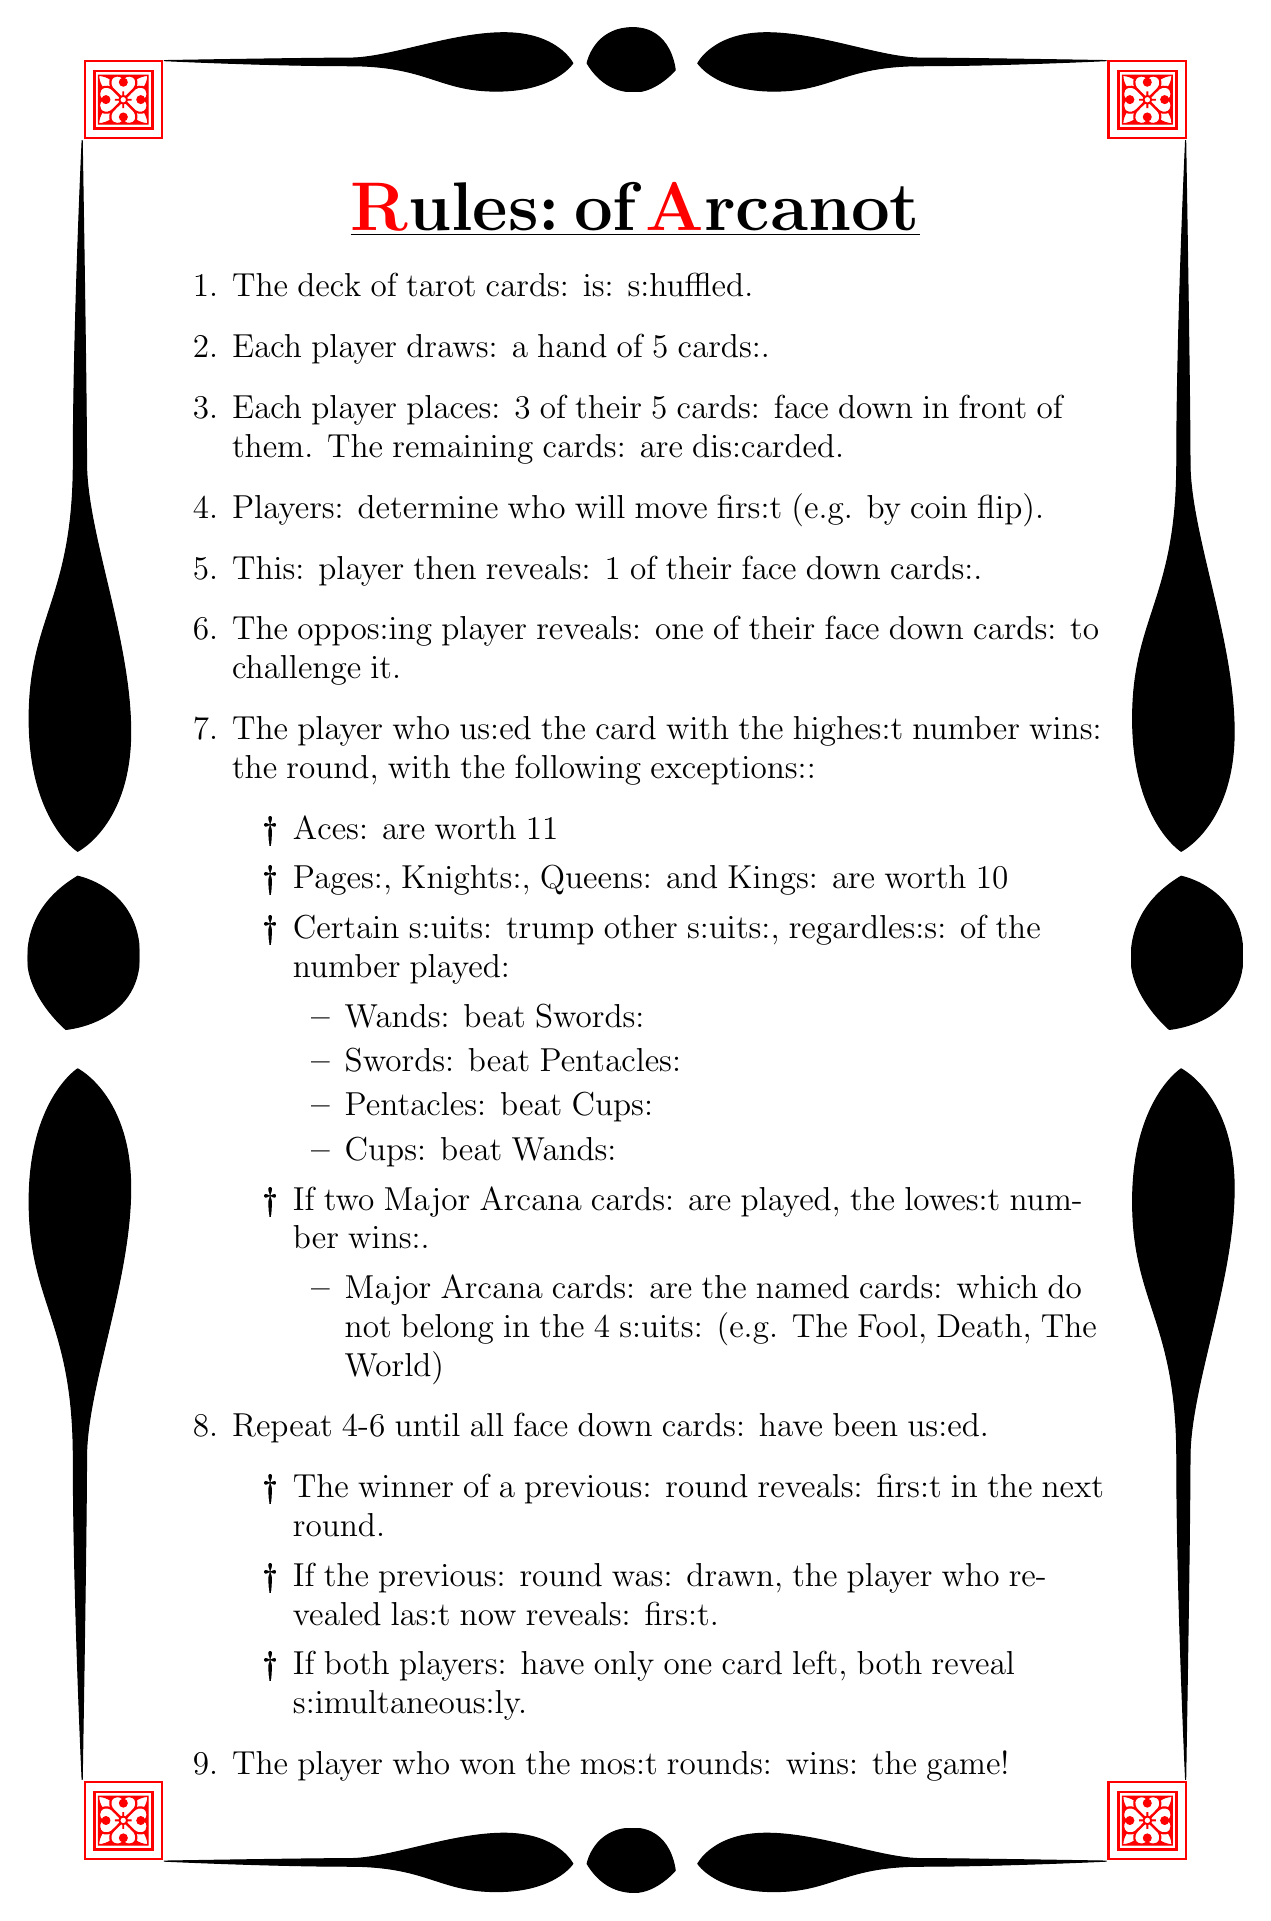
\begin{tikzpicture}[every node/.style={inner sep=0pt}]
   \node[text width=12cm,align=center](Text){%
   \section*{\textgoth{\Huge\underline{\textcolor{red}{R}ules: of \textcolor{red}{A}rcanot}}}

{\swabfamily\fraklines\large
\begin{enumerate}
   \item The dec\textgoth{k} of tarot cards: is: s:huffled.
   \item Each player draws: a hand of 5 cards:.
   \item Each player places: 3 of their 5 cards: face down in front of them. The remaining cards: are dis:carded.
   \item Players: determine who will move firs:t (e.g. by coin flip).
   \item This: player then reveals: 1 of their face down cards:.
   \item The oppos:ing player reveals: one of their face down cards: to challenge it.
   \item The player who us:ed the card with the highes:t number wins: the round, with the following exceptions:: 
      \begin{itemize}
         \item Aces: are worth 11
         \item Pages:, Knights:, Queens: and Kings: are worth 10
         \item Certain s:uits: trump other s:uits:, regardles:s: of the number played:
            \begin{itemize}
               \item Wands: beat Swords:
               \item Swords: beat Pentacles:
               \item Pentacles: beat Cups:
               \item Cups: beat Wands:
            \end{itemize}
         \item If two Major Arcana cards: are played, the lowes:t number wins:.
            \begin{itemize}
               \item Major Arcana cards: are the named cards: which do not belong in the 4 s:uits: (e.g. The Fool, Death, The World)
            \end{itemize}
      \end{itemize}
   \item Repeat 4-6 until all face down cards: have been us:ed.
   \begin{itemize}
      \item The winner of a previous: round reveals: firs:t in the next round.
      \item If the previous: round was: drawn, the player who revealed las:t now reveals: firs:t.
      \item If both players: have only one card left, both reveal s:imultaneous:ly.
   \end{itemize}
   \item The player who won the mos:t rounds: wins: the game!
\end{enumerate}
}} ;
   \node[shift={(-1cm,1cm)},anchor=north west](CNW)
   at (Text.north west) {\pgfornament[color=red,width=1cm]{7}};
   \node[shift={(1cm,1cm)},anchor=north east](CNE)
   at (Text.north east) {\pgfornament[color=red,width=1cm,symmetry=v]{7}};
   \node[shift={(-1cm,-1cm)},anchor=south west](CSW)
   at (Text.south west) {\pgfornament[color=red,width=1cm,symmetry=h]{7}};
   \node[shift={(1cm,-1cm)},anchor=south east](CSE)
   at (Text.south east) {\pgfornament[color=red,width=1cm,symmetry=c]{7}};
   \pgfornamenthline{CNW}{CNE}{north}{80}
   \pgfornamenthline{CSW}{CSE}{south}{80}
   \pgfornamentvline{CNW}{CSW}{west}{80}
   \pgfornamentvline{CNE}{CSE}{east}{80}
   \end{tikzpicture}

\end{document}